%!TEX root = ../main/main.tex

Un \href{https://en.wikipedia.org/wiki/Merkle_tree}{árbol de Merkle} es una estructura de datos que utiliza una función de hash criptográfica $h$ para representar un conjunto de strings $S=\{s_1,\ldots,s_m\}$. La estructura es un árbol binario en el que cada nodo es un string definido recursivamente: Las hojas son $h(s_1),\ldots,h(s_m)$ y cada nodo interior $n$ se define como $h(n_1 \| n_2)$ donde $n_1$ y $n_2$ son los hijos de $n$ y $\|$ representa la concatenación de strings. Cuando la cantidad de nodos en un nivel es impar se duplica el último nodo de dicho nivel, lo que implica que todos los nodos interiores tienen exactamente dos hijos. La Figura~\ref{fig:merkle} muestra gráficamente la construcción de un árbol de Merkle:

\begin{figure}[h]
  \scriptsize
  \begin{center}
    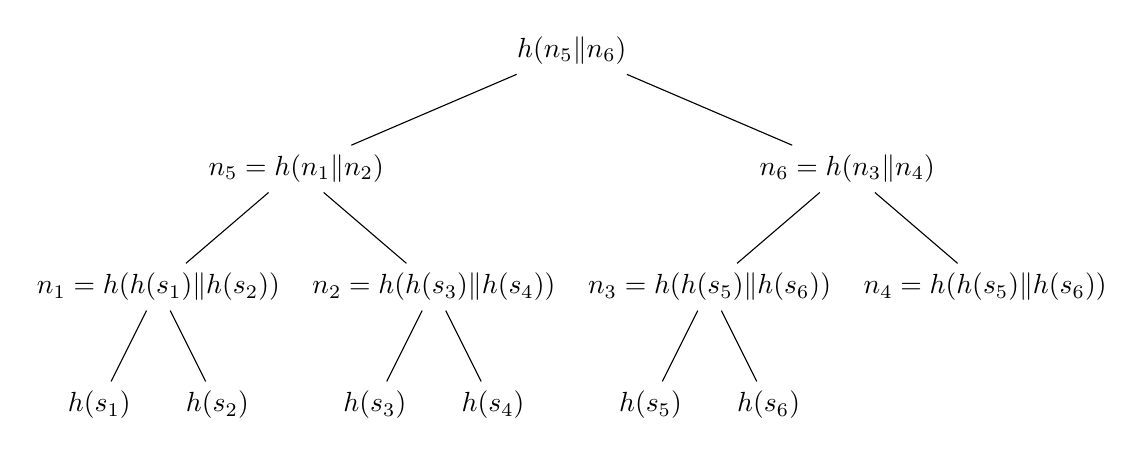
\begin{tikzpicture}[
      level distance=1.5cm,
      level 1/.style={sibling distance=7cm},
      level 2/.style={sibling distance=3.5cm},
      level 3/.style={sibling distance=1.5cm}
    ]
    \node{$h(n_5\|n_6)$}
    child {
      node{$n_5=h(n_1\|n_2)$}
        child {
          node {$n_1=h(h(s_1)\|h(s_2))$}
          child {
            node {$h(s_1)$}
          }
          child {
            node {$h(s_2)$}
          }
        }
        child {
          node {$n_2=h(h(s_3)\|h(s_4))$}
          child {
            node {$h(s_3)$}
          }
          child {
            node {$h(s_4)$}
          }
        }
      }
      child{
        node{$n_6=h(n_3\|n_4)$}
        child{
          node {$n_3=h(h(s_5)\|h(s_6))$}
          child{
            node{$h(s_5)$}
          }
          child{
            node{$h(s_6)$}
          }
        }
        child{
          node {$n_4=h(h(s_5)\|h(s_6))$}
        }
      }

      ;
    \end{tikzpicture}
  \end{center}
  % \includegraphics[width=\linewidth]{../images/merkle_tree.jpeg}
  \caption{Árbol de Merkle para el conjunto $S=\{s_1,\ldots,s_6\}$.}
  \label{fig:merkle}
\end{figure}

La principal propiedad de un árbol de Merkle es que si una persona posee un hash que representa la raíz del árbol, la podemos convencer rápidamente de que un elemento es una de las hojas del árbol. Para esto, basta con compartir con esa persona dicho elemento, su hermano y los hermanos de todos sus ancestros, indicando para cada uno si es hermano derecho ($d$) o izquierdo ($i$). Por ejemplo, supongamos que alguien tiene la raíz del árbol que se muestra en la Figura~\ref{fig:merkle}. Para convencer a dicha persona de que $s_5$ es parte del conjunto $S$ basta con enviarle el valor $s_5$ junto con $(h(s_6),d)$, $(n_4,d)$ y $(n_5,i)$. Teniendo estos valores, esta persona puede:

\begin{itemize}
  \item Computar $n_3=h(h(s_5)\|h(s_6))$.
  \item Computar $n_6=h(n_3\|n_4)$.
  \item Computar $h(n_5\|n_6)$ y verificar que el resultado sea igual a la raíz del árbol.
\end{itemize}

En esta pregunta usted deberá programar una clase que permita crear árboles de Merkle para conjuntos arbitrarios de strings, usando una función de hash arbitraria. Deberá seguir las instrucciones indicadas más arriba, entregando un Jupyter Notebook que define una clase como la siguiente:

\bigskip
\begin{python}
  class MerkleTree:
    
    def __init__(self, strings: [str], hash_func: (str) -> str) -> MerkleTree:
    """
    Arguments:
      strings: The set of strings S
    """

    def get_root(self) -> string:
    """
    Returns:
      root: Root of the Merkle Tree
    """

    def get_proof_for(self, item: str) -> None || [(str, "d"|"i")]:
    """
    Returns:
      result: None if the item is not part of the leafs of the tree
              A list with the necessary info to prove that the
              item is part of the leafs of the tree
    """
\end{python}

Además de esta clase, usted deberá programar una función que reciba una \emph{prueba} de que un elemento es parte de un árbol de Merkle, y retorne \texttt{True} si la prueba es correcta y \texttt{False} de lo contrario. Esta función también deberá estar escrita en su Jupyter Notebook y deberá tener la siguiente firma:

\bigskip
\begin{python}
  def verify(root: string, item: str, proof: [(str, "d"|"i")], hash_func: (str) -> str) -> bool:
    """
    Arguments:
      root: The root of a merkle tree
      item: An abritrary string
      proof: An alleged proof that item is part of a Merkle
             tree with root root
      hash_func: An arbitrary hash function
    Returns:
      correct: whether the proof is correct or not
    """
\end{python}
